\begin{refsection}
\chapter{Kernels}

\begin{summary}
Machine learning often considers problems where we profile objects with attribute-value vectors. This representation has, in principle, several limitations. Objects may be complex, and their vector-based representation is not trivial. Consider text documents, molecular structures, trees, graphs, and networks. For these, an alternative to feature-based representation is the utility of a function that can measure object-to-object similarity. Moreover, even if feature-based representation is available, it may be too weak to allow simpler models, like linear and logistic regression, to model more complex relations, like feature interactions. One way to surpass such limitations is kernels. In general, kernels are functions that map a pair of input objects to a number. One use of kernels is to consider a prototype object and then map input space into a latent representation, where selected modeling techniques may be more successful. When applied to a pair of data instances, we can regard kernels as functions that measure similarity. Smoothing kernels as used in kernel density estimation, which has a substantially different meaning. In this chapter, we look at a range of typical kernels and approaches that can use kernels in model inference.
\end{summary}

In the previous chapters, we have introduced machine learning models that consider a set of training data to infer a predictive model. The training data is then discarded, and predictions for new inputs are formed entirely based on the model and its inferred parameters. 

In this chapter, we introduce a different class of machine learning techniques that keeps the training data and uses it within the prediction phase. We have already exposed one such algorithm, namely $k$-nearest neighbors. We refer to algorithms of this kind as {\em lazy}, or {\em memory-based}. They typically require a metric of similarity of any two data points from the input space. We can recast many linear parametric models into an equivalent dual representation in which the predictions are based on a linear combination of a {\em kernel function} evaluated in the original, input space. For models, which are based on a fixed non-linear {\em feature space mapping} $\phi$, the kernel function is given by the relation
$$ \kappa(\x,\x')=\phi(\x)^\tr \phi(\x').$$
The kernel function is, from the definition, symmetric. Again, and importantly, the definition above says that instead of computing the dot product between the vectors in the latent, mapped space, we can compute the kernel function in the space of original features.  This concept, thus formulated as an inner product in a feature space, allows us to develop extensions of many well-known regression and classification methods. All we need to do is to reformulate the methods to operate with dot products of input vectors. When introducing transformation to latent space, this product is then replaced with the kernel. We show the utility of the kernel trick in detail for one regression and for one classification approach: linear regression with ridge regularization and support vector machines. 

In particular, support vector machines have received much attention in the past, but their importance has been in decay with the introduction of recent approaches, including deep networks. A particularly important driver of support vector machine's success was the utility of kernels on structured objects, like text, voice, images, and graphs.

\section{Examples of Kernel Functions}

A {\em kernel function}, or just a {\em kernel} is defined as:
$$\kappa: \mathcal{X} \times \mathcal{X} \rightarrow \mathbb{R},$$
where $\mathcal{X}$ is our variable space or typically, an input space. A kernel is thus a function $\kappa(x, x')$ that takes a pair of elements from the input space $x, x' \in \mathcal{X}$ and maps them to a real number. In practice we typically deal with kernel functions where $\kappa(x, x') \geq 0$ and $\kappa(x, x') = \kappa(x', x)$. That is, non-negative and symmetric kernel functions, which allows us to interpret them as \emph{similarity measures}. 

Notice that \emph{kernel} has different meanings in different contexts. We will be here covering three:

\begin{itemize}
\item First, we will look at kernels in a very general sense - as functions that map a pair of elements from our (input, feature) space to a number.
\item Then we will move on to positive-definite (or Mercer) kernels, which are a special case of the former (that is, with additional requirements) and allow for more efficient computation that is the basis for models such as SVM and kernel ridge regression.
\item And third, we will introduce smoothing kernels that are used in kernel density estimation and has a substantially different meaning.
\end{itemize}

\subsection*{Polynomial Kernel}

A standard kernel that is related to a transformation to a latent space that can, for instance, yield a linearly-unserable data instances manageble under linear models (e.g., Fig.~\ref{fig:svm-circle}) is a polynomial kernel:
$$ \kappa(\x,\x')=(\x^\tr \x'+1)^n.$$
For $n=2$, and assuming that $x=[u_1 u_2]^\tr$ and $x'=[v_1 v_2]^\tr$ we get
\begin{align*}
(\x^\tr \x'+1)^2 & = (u_1 v_1 + u_2 v_2 +1)^2 \\
& = u_1^2 v_1^2 + u_2^2 v_2^2 + 1 + 2 u_1 v_1 + 2 u_2 v_2 + 2 u_1 v_1 u_2 v_2 \\
& = \langle 1, \sqrt{2}\ u_1, \sqrt{2}\ u_2, u_1^2, \sqrt{2}\ u_1 u_2, u_2^2\rangle^\tr  \langle 1, \sqrt{2}\ v_1, \sqrt{2}\ v_2, v_1^2, \sqrt{2}\ v_1 v_2, v_2^2\rangle
\end{align*}

Polynomial kernel of second degree returns a dot product of vectors in six-dimensional space.

\subsection*{Radial Basis Function Kernels}

The squared exponential kernel, or {\em Gaussian} kernel is defined by:
$$ \kappa(\x, \x')=\exp\left( -{1\over 2}(\x-\x')^\tr\Sigma^{-1}(\x-\x') \right) $$
When $\Sigma$ is diagonal, this kernel can be expressed as:
$$ \kappa(\x,\x')=\exp\left(-{1\over 2}\sum_{j=1}^D {1\over\sigma_j^2}(x_j-x_j')^2 \right) $$
We can interpret $\sigma_j$ as characteristic lenght scale of the dimension. If we assume that all characteristic length scales are equal, then we can write this kernel as:
$$ \kappa(\x,\x')=\exp\left( - {\norm{\x-\x'}^2\over 2\sigma^2}\right) $$
where $\sigma^2$ is known as a bandwidth. Since this kernel depends only on a function $\norm{\x-\x'}$, that is, only on a distance between a point $\x$ and, say, a reference $\x'$, this kernel is a radial basis function and is often referred to as an {\em RBF kernel}.

Notice that an RBF kernel has a parameter, $\sigma$, that needs to be either set by the user given some domain knowledge or inferred from the data through, for example, internal cross-validation.

\subsection*{Linear Kernel}

When $\phi(\x)=\x$, we get a linear kernel defined as:
$$ \kappa(\x,\x')=\x^\tr x' $$

This kernel is useful if the original data is already high dimensional, and if the original set of features are informative. Examples of such data sets are frequent in text mining and related with a bag of words representation of text documents, or data set from molecular biology that involve thousands of genes or millions of single-nucleotide polymorphisms. In these cases, a linear combination of features may represent a sufficiently accurate decision boundary, and it may not be required to use some other latent representation.

\subsection*{Kernels for Comparing Text Documents}

Notice that kernel provides a proxy for the similarity of data instances. Given two objects, we will be able to construct regressors or classifiers by only computing the kernels, that is, estimating the similarity between two objects. If the objects are text documents, we can represent the document with vectors that contain word frequencies. We often refer to this presentation as {\em bag of words}. Because we can consider documents of different lengths, the Euclidian distance would fail (why?). We can instead normalize the bag-of-words representation according to the document length or use the {\em cosine similarity}~\footnote{Euclidian distance between normalized vectors and cosine similarity are in practice almost identical. Find what is their relation mathematically!}:
$$ \kappa(\x, \x')= {\x^\tr \x'\over\norm{\x}\norm{\x'}}  $$
Cosine similarity measures the cosine of the angle between the two vectors $\x$ and $\x'$ that represent the corresponding documents. Since both vectors are count vectors, the cosine similarity will be between 0 and 1. 

Bag of words representation may include punctuations and frequently occurring words, so-called stop words, that may obscure the differences between documents and yield document representations too similar to each other. Various techniques for text pre-processing to avoid this effect were proposed in the literature. Among the most frequently used are stop-words removal and transform called {\em term frequency-inverse document frequency}, which replaces word counts with weights so that to expose less frequent words.

\subsection*{String Kernels}

Kernels that operate on strings report on string sequence similarity. In these times, it may not be hard to consider RNA sequences of viruses that have infected people at different continents. Due to mutations, their sequence may be different, and so is the effect on a phenotype of a patient. We may predict these phenotypes using kernels that measure sequence similarity. Consider the following three sequences:
\begin{verbatim}
TCGGTTTAACGGATTATGGTAC
TCGGTCCAACGGATAATGGAAC
TCGGCGATTTAACGGATCGATTTATGGTAC
\end{verbatim}
To compare them, we may, for instance, use edit distance, that is, the measure that reports how many atomic changes like deletions, insertion, or single nucleotide mutation we have to introduce in one sequence to derive another one. Sequence similarity may also be computed through the count of the substrings the two strings have in common, or through the length of the longest common substring, or similar. There is vast research on string similarity measures and means to compute them through sequence alignment in the literature of molecular biology, and interested readers should consult algorithms such as BLAST or CLUSTAL.

\section{Kernelized Linear Models}
% entire 14.3

One simple way to use kernels for classification or regression is to use {\em kernel machines}. A kernel machine is a generalized linear model where the input vector has the form
$$ \phi(\x)=[\kappa(\x,\vect{\mu_1}), \ldots, \kappa(\x,\vect{\mu_K}) ] $$
where $\vect{\mu}_k$ is a set of {\em centroids} or {\em prototypes}, that is, a subset of examples from the training set. Considering kernels as proximity functions. Then, the above-defined {\em kernelized feature vector} can be, for a give data instance, regarded as a vector of similarity to the prototype data instances. The general idea is that wherever we use a linear term $\b^T\x$, that is, in linear regression, generalized linear models, ordinal regression or similar, we could instead transform the input vector $x$ via a kernel function with respect to a set of \emph{prototype} observations $\vect{\mu}_1$, ..., $\vect{\mu}_k$. After constructing these new features, we proceed with the inference as we would with the original modeling method, we have a different, transformed input space (the term used now is $\beta^T\phi(x)$.

Prototypes, if appropriately selected, may help linear models to model feature spaces with feature interactions. Consider an XOR problem and logistic regression. Using RBF kernel and four different prototypes, logistic regression would be able to infer a perfect model for this otherwise hard classification case. Notice, though, that choice of the prototypes here is essential. In general, though:
\begin{itemize}
\item The number of prototypes $K$ can be less, above, or equal to the dimension of the original training set.
\item We can choose the prototypes using some systematic approach, like clustering. Alternatively, we could use every training example, $x$, for a prototype.
\item If the number of prototypes is large, we could use any of the sparsity-promoting priors on $\b$, as discussed in the chapter on regularization. We refer to such an approach is called {\em sparse vector machine}. The most natural choice is $\ell_1$ regularization, an approach we refer to as {\em $\ell_1$-regularized vector machine}, or L1VM. Another popular approach of creating a sparse kernel machine is a support vector machine, discussed in detail below.
\item And, most importantly, worth emphasizing again -- we can use this approach within any linear model we have learned so far. With this approach, we can produce non-parametric versions of those parametric approaches, where their expressiveness can grow with the number of data points.
\end{itemize}


\section{Mercer Kernels}

Mercer kernels are related to approaches that use kernels through the so-called kernel trick and where we define models where input data appears within the inner products of the input data instances. We here define the Mercer kernels, establish the equivalence between Mercer kernels and inner products in transformed space, and outline some of the rules to follow when constructing a new kernel.

\subsection*{Definition Mercer's Theorem}
% 14.2.3 for reference, but our treatment is better structured

A kernel function $\kappa$ of the form $\mathbb{R}^d \times \mathbb{R}^d \rightarrow \mathbb{R}$ is said to be \textit{symmetric positive semidefinite} if it is (a) symmetric: $\kappa(x, x') = \kappa(x', x)$ and (b) for any integer $m > 0$ and any set of $m$ vectors $x_i \in \mathbb{R}^d$ the matrix
%
$$ K = 
\begin{bmatrix} 
    \kappa(x_1,x_1) & \hdots & \kappa(x_1,x_m) \\
    \vdots & \ddots & \vdots \\
    \kappa(x_m,x_1) & \hdots & \kappa(x_m,x_m) \\
\end{bmatrix} $$
is positive semidefinite. This matrix is also called the \emph{Gram} matrix.

\begin{definition}{Mercer Kernel.}
A symmetric positive semidefinite kernel $\kappa$ is also called a \emph{Mercer kernel}.
\end{definition}

\begin{definition}{Mercer's Theorem.}
If $\kappa$ is a Mercer kernel then it is an inner product (dot product) $\kappa(x, x') = \langle\phi(x), \phi(x')\rangle$ for some (possibly infinite dimensional) mapping $\phi(x): \mathbb{R}^m \rightarrow \mathcal{D}$.
\end{definition}

Note that the mapping $\phi$ is often called the \emph{basis function} and the space $\mathcal{D}$ is called the $\emph{feature space}$.

This theorem is fundamental. It justifies the \emph{kernel trick} that we will see a couple of times later. The kernel trick is just a direct application of Mercer's theorem - if we have a method that depends only on the inner products, we can replace those inner products with any Mercer kernel to obtain the application of that method on the feature space $\mathcal{D}$ determined by that kernel. Of course, computing the kernel is, in most cases, much easier.


\subsection*{Polynomial Kernel Revisited}
% 14.2.3 but we take a more simple stand-alone approach and focus on the essentials

We can start by considering one-dimensional polynomial regression, which is equivalent to using the basis function $\phi: x \rightarrow (1, x, x^2, ..., x^r)$. For example, for quadratic polynomial regression ($r = 2$), $\phi: x \rightarrow (1, x, x^2)$ and for cubic polynomial regression ($r = 3$), $\phi: x \rightarrow (1, x, x^2, x^3)$. Similarly, for higher dimensional $x$, we have $\phi: (x_1, x_2) \rightarrow (1, x_1, x_2, x_1x_2, x_1^2, x_2^2)$.

In practice, it turns out that the basis functions for polynomial kernels use slightly different weights. For the cubic example, instead of $\phi: x \rightarrow (1, x, x^2, x^3)$, we use $\phi: x \rightarrow (1, \sqrt{3}x, \sqrt{3}x^2, x^3)$. The squared-roots do not make any difference when considering linear combinations, as the inner two coefficients will just be scaled by $\sqrt{3}$. However, it does make the computation much more convenient:

$$\langle\phi(x), \phi(x')\rangle = 1 + 3xx' + 3x^2(x')^2 + x^3(x')^3 = (1 + xx')^3.$$

This can be generalized to arbitrary power $r$, obtaining the {\em polynomial kernel} $\kappa(x,x') = (1 + xx')^r$. The beauty of this kernel is that the computation of the inner product in feature space, which has ${r+m}\choose{m}$ dimensions, actually requires just one inner product in the original space (dimension $m$) adding one and taking power.

\subsection*{RBF Kernel Revisited}

With no proof, we should state here that:
\begin{enumerate}
\item Radial basis function (RBF) kernel is a Mercer kernel.
\item RBF kernel corresponds to a basis function that transforms the data instance to an infinite-dimensional feature space, that is, to a space of an infinite sum of polynomial kernels. So not only is the feature space inner product more convenient to compute in original space, it would be impossible to compute in feature space.
\end{enumerate}

% \subsection*{Matern kernel (14.5.2)}

% This kernel is also a Mercer kernel is very popular in Gaussian Processes. We can mention it here or when we do Gaussian Processes.

\subsection*{Other Mercer Kernels}

In general, it is difficult to verify if a kernel is a Mercer kernel. There are, however, operations that preserve the property. If $\kappa_1$ and $\kappa_2$ are Mercer kernels defined on the same feature space, then the following are also Mercer kernels~\citep{ShaweTaylorCristianini2004}:

\begin{itemize}
    \item $\kappa(x, x') = c\kappa_1(\x,\x')$, where $c>0$ is a constant
    \item $\kappa(x, x') = f(\x)\kappa_1(\x, \x')f(\x')$, where $f(x)$ is a real function with nonnegative coefficients
    \item $\kappa(x, x') = f(\kappa_1(\x, \x'))$
    \item $\kappa(x, x') = \kappa_1(\x, \x') + \kappa_2(\x,\x')$
    \item $\kappa(x, x') = \kappa_1(\x, \x')\kappa_2(\x,\x')$
    \item $\kappa(x, x') = \kappa_1(\phi(\x),\phi(\x'))$
    \item $\kappa(x, x') = \x^\tr \matr{A}\x'$, where $\matr{A}$ is symmetric positive semidefinite matrix
\end{itemize}

Let us start with a linear function $\kappa(\x,\x')=(\x^\tr \x')$, which is a kernel since $\matr{A}=\matr{I}$ is a positive definite matrix, (and as such also positive semi-definite). Then a simple polynomial kernel $\kappa(\x,\x')=(\x^\tr \x')^2=$ contains only terms of degree two, and is equal to the linear kernel squared, and is also a kernel. A slightly generalized function $\kappa(\x,\x')=(\x^\tr \x'+c)^2$ with $c>0$ is also a kernel since its expansion contains linear combinations of linear or polynomial kernels of degree two. Through similar reasoning, we can find taht $\kappa(\x,\x')=(\x^\tr \x'+c)^M$ is a kernel for any $c\geq 0$.

Another commonly used kernel, a Gaussian kernel, takes the form
$$ \kappa(\x, \x')=\exp\left(-\norm{\x-\x'}^2/2\sigma^2 \right) $$
This is a valid kernel, sinceby expanding the square
$$ \norm{\x-\x'}^2=\x^\tr\x + (\x')^\tr\x' - 2\x^\tr \x' $$
we can write
$$ \kappa(\x, \x')=\exp(-\x^\tr\x/2\sigma^2) \exp(\x^\tr\x'/\sigma^2) \exp(-(\x')^\tr\x'/ x\sigma^2) $$
and see that this is a valid kernel.

\section{Application of the Theory of Mercer Kernels to Modelling}

We want to express an existing linear method in terms of inner products and then replace them with a kernel to obtain the linear method in the transformed feature space, consequently constructing a non-linear model. That is, we apply the \emph{kernel trick}. Of course, for this to work, the kernel needs to be a Mercer kernel, not just any kernel function. Below, we show that regularized linear regression has a dual form that uses dot products of input vectors, and hence it can be kernelized. We also derive support vector machines, a linear classification algorithm that uses a weighted sum of the dot product of pairs of data instances from the training data set. Furthermore, we briefly discuss a kernelized version of the $k$-nearest neighbors. For other methods, like support vector machine regression, kernelized principal component analysis, or kernelized $k$-means clustering, see \citep{2012-Murphy}.

\subsection*{Kernelized Ridge Regression and the Kernel Trick}

First, recall what we've learned about ridge regression, that is, L$_2$-regularized linear regression. Again, let $X \in \mathbb{R}^{N \times D}$ be our independent variables and $y \in \mathbb{R}^N$ our dependent variable. Given a regularization parameter $\lambda$ the objective is to find coefficients $\beta$ that minimize the squared error and the squared sum of coefficients $\beta$,

$$\hat{\beta} = \arg \min_\beta \left(\lvert\lvert X\beta - y  \rvert\rvert_2^2  + \lambda \lvert\lvert \beta  \rvert\rvert_2^2\right).$$

We know that this has a closed-form solution $\hat{\beta} = (X^TX + \lambda I_d)^{-1}X^Ty$.

Now we will rewrite this solution in an alternative (dual) form, which will facilitate the use of a kernel. Observe that

$$(X^TX + \lambda I_d)X^T = X^TXX^T + \lambda X^T = X^T(XX^T + \lambda I_n).$$

Multiplying the leftmost and rightmost terms by $(X^TX + \lambda I_d)^{-1}$ on the left and $(XX^T + \lambda I_d)^{-1}$ on the right-hand side, we get

$$X^T(XX^T + \lambda I_n)^{-1} = (X^TX + \lambda I_d)^{-1}X^T.$$

So, we have found an alternative formulation of the closed-form solution:

$$\hat{\beta} = X^T(XX^T + \lambda I_n)^{-1}y.$$

Using this new formulation as depicted above, we can define the prediction for a new observation as

$$\hat{y}(x') = \hat{\beta}^Tx' = (x')^T\hat{\beta} = (x')^T X^T(XX^T + \lambda I_n)^{-1}y.$$

The critical observation here is that {\em the prediction depends on $X$ and $x'$ only through standard inner products}.

More precisely, $(x')^T X^T = \begin{bmatrix} 
\langle x',x_1 \rangle \\
 \vdots \\ 
\langle x',x_n \rangle  \\  \end{bmatrix}^T $ and $XX^T =  \begin{bmatrix} 
\langle x_1,x_1 \rangle & \hdots & \langle x_1,x_n \rangle \\
 \vdots & \ddots & \vdots \\ 
  \langle x_n,x_1 \rangle & \hdots & \langle x_n,x_n \rangle \\  \end{bmatrix} $ is the Gram matrix.

So, we can apply the \emph{kernel} trick and replace these inner products with the more general kernelized formulation.

$$\hat{y}(x') = k(x')(K + \lambda I_n)^{-1}y,$$
%
where $k(x') = \begin{bmatrix} 
\kappa(x',x_1) \\
 \vdots \\ 
\kappa(x',x_n) \\  \end{bmatrix}^T $ and $K = \begin{bmatrix} 
\kappa(x_1,x_1) & \hdots & \kappa(x_1,x_n) \\
 \vdots & \ddots & \vdots \\ 
 \kappa(x_n,x_1) & \hdots & \kappa(x_n,x_n) \\  \end{bmatrix}. $
 
That is, using a kernel, we can perform ridge regression in the space whose inner product is represented by the kernel.

An alternative view is to explicitly introduce the (dual) variable $\alpha = (K + \lambda I_n)^{-1}y$ to allow us to express the closed-form solution as

$$\hat{\beta} = X^T\alpha = \sum \alpha_i x_i.$$
%
The solution to the problem is just a linear combination of the observations!

Plugging this into the prediction for the new observation, we get

$$\hat{y}(x') = (x')^T \sum \alpha_i x_i  =  \sum \alpha_i (x')^T x_i = \sum \alpha_i \kappa(x',x_i),$$
%
which illustrates that the prediction for a new observation is just a weighted sum of training observations' values of $y$ (weighted by the similarity of those observations with the new observation $x'$)! For example, for linear regression, where we just have the standard inner product, observations that have a smaller angle (closer to 0 or 180) have a higher weight.

The degree of fit of kernelized ridge regression depends on the choice of kernel and its parameters, and on the choice of degree of regularization (see Figs.~\ref{fig:kernels-poly} and \ref{fig:kernels-rbf}).

\begin{figure}
\centering{
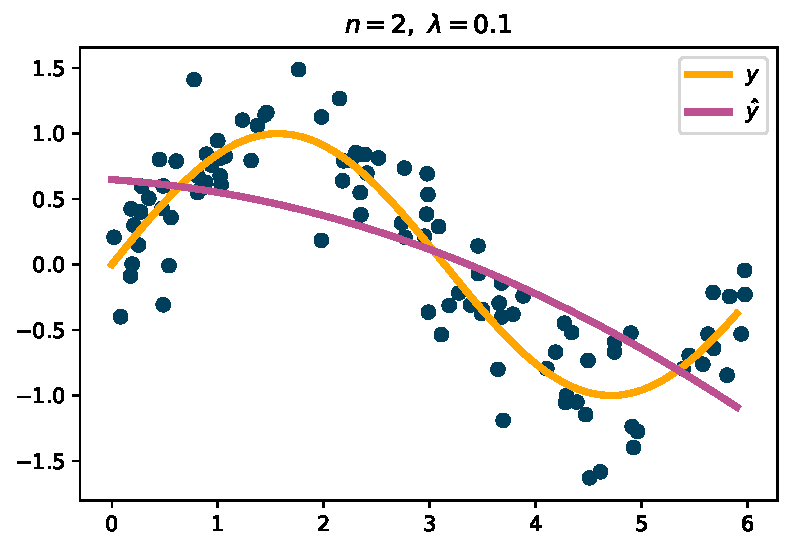
\includegraphics[width=0.47\linewidth]{figures/kernels-sin-poly-2.pdf}
\hfill
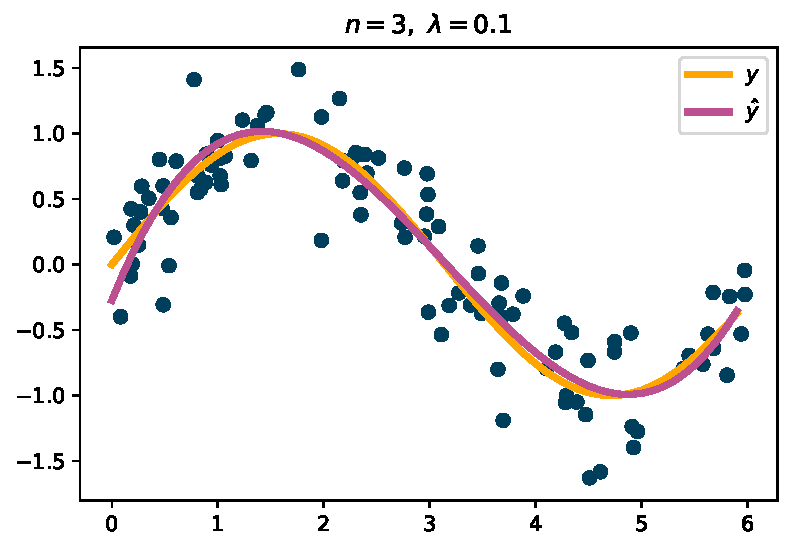
\includegraphics[width=0.47\linewidth]{figures/kernels-sin-poly-3.pdf}
}
\caption{Kernelized ridge regression with polynomial kernel on one-dimensional data. Choice of hyper-parameter of the kernel can greatly influence the degree of fit.}
\label{fig:kernels-poly}
\end{figure}

\begin{figure}
\centering{
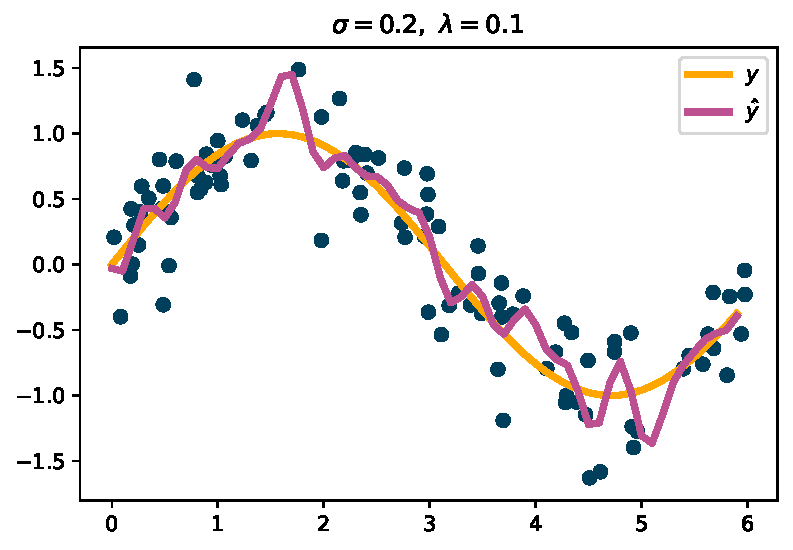
\includegraphics[width=0.47\linewidth]{figures/kernels-sin-rbf-02.pdf}
\hfill
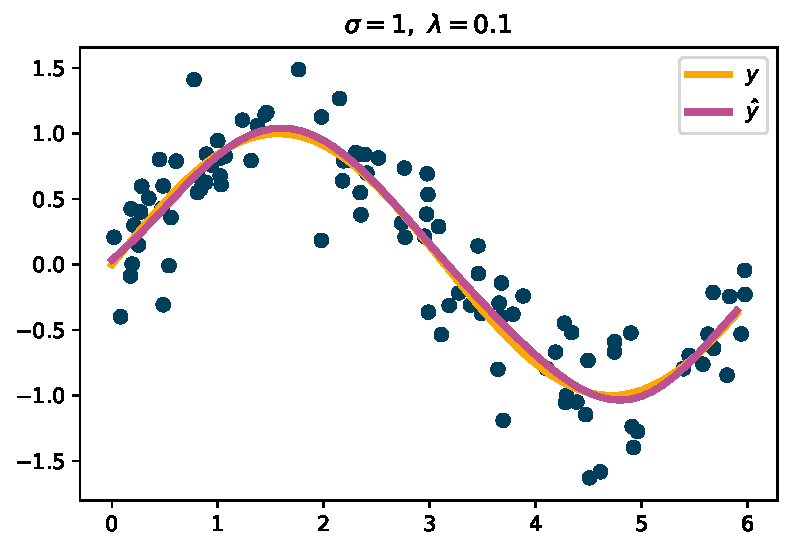
\includegraphics[width=0.47\linewidth]{figures/kernels-sin-rbf-10.pdf}
}
\caption{Wrong choice of hyperparameters can lead to overfitting, as shown in the plots of regression on one-dimensional data set with Gaussian kernel.}
\label{fig:kernels-poly}
\end{figure}

\subsection*{Support Vector Machines}

Support vector machines are, in essence, linear classifiers that infer separating hyper-planes with maximal margins to the neighboring data points. We here derive the formulation of this classifier, show how to its power with a kernel trick, and describe extension for non-linearly separable cases. We also derive the formulation for support vector machines using hinge loss.

\subsubsection*{The Large Margin Principle}

\begin{figure}[htbp]
\centering{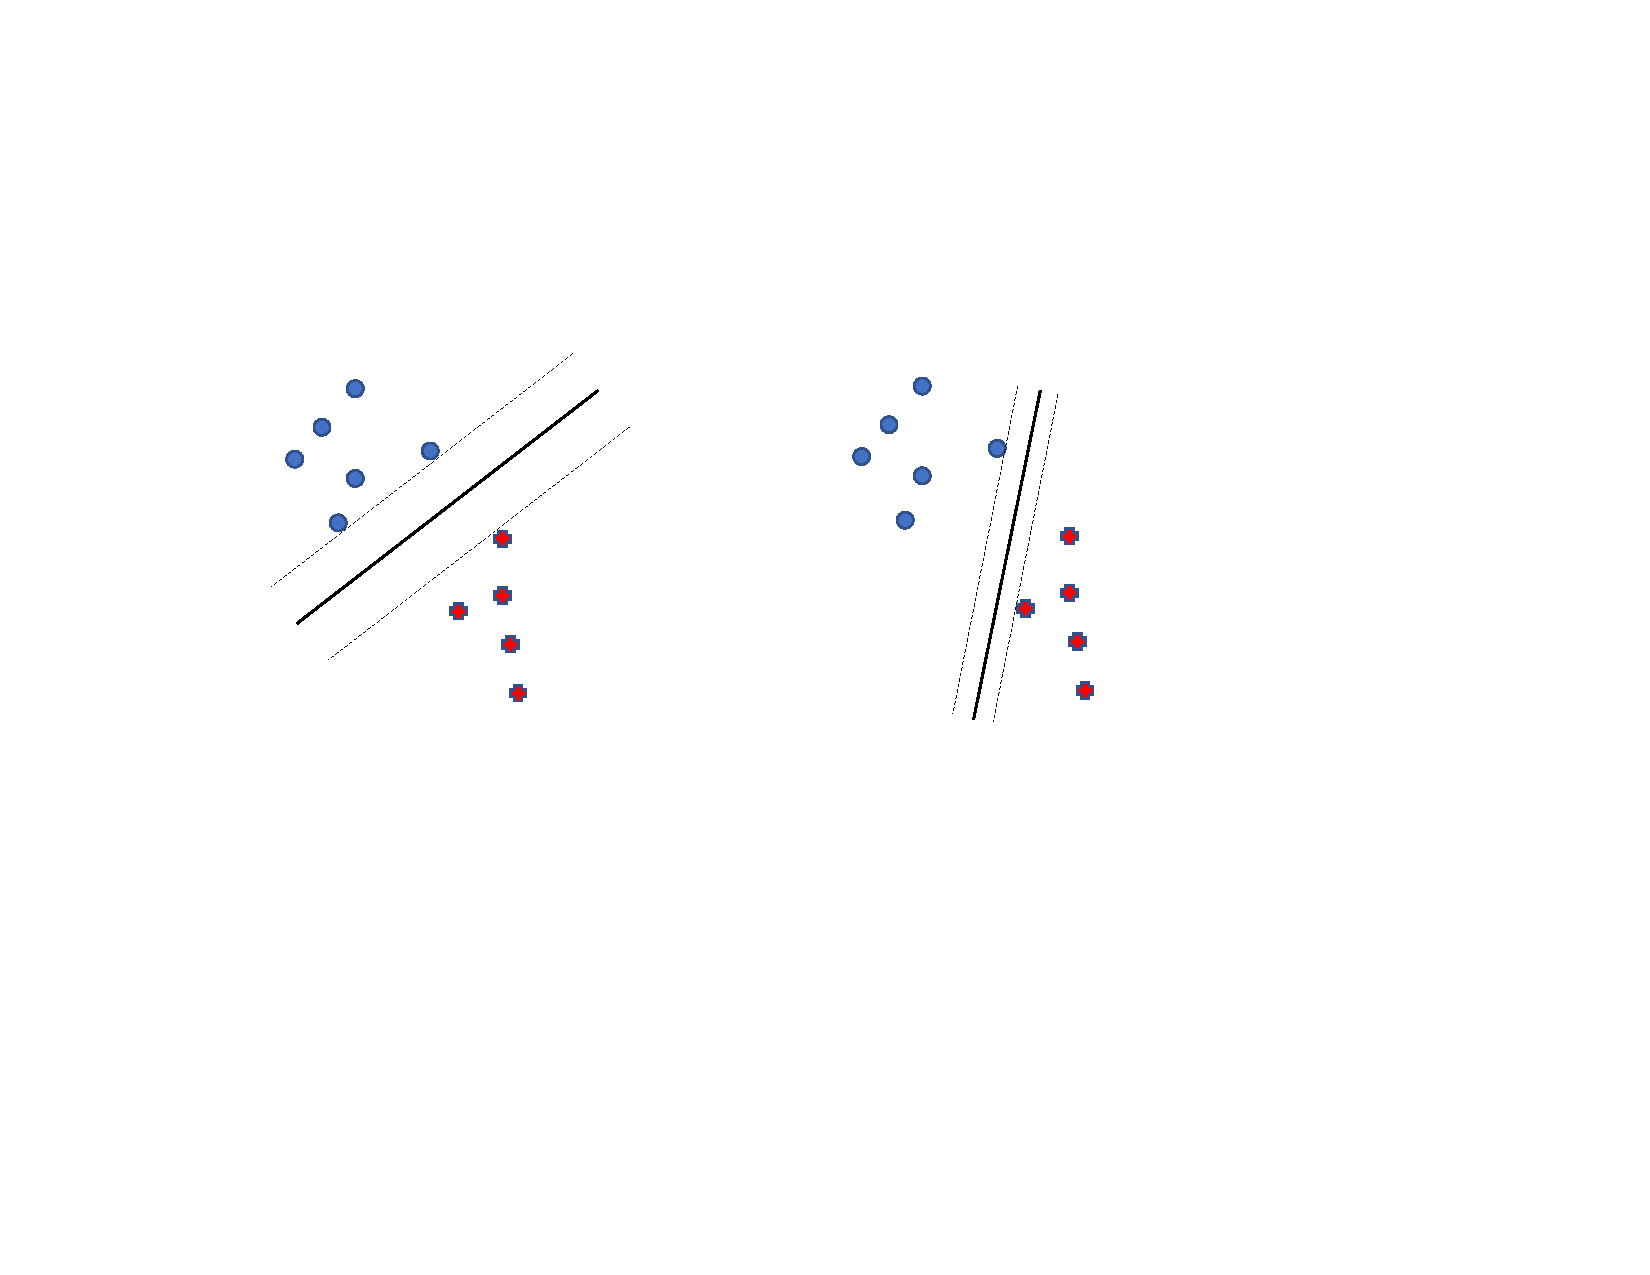
\includegraphics[width=12cm]{figures/kernels-margin.pdf}}
%TODO
\caption{A separating hyper-plane with large (left) and small margin (right).}
\label{fig:svm-lin-sep}
\end{figure}

Consider a binary classification problem, with $y=\pm 1$, where data instances of the two classes are linearly separable. Our aim is to define a separating hyper-plane that splits the feature space so that the margin between the closest positive and the closest negative data instance is the largest~\ref{fig:svm-lin-sep}. Intuitively, a large margin would steer us from overfitting and may yield best accuracy on yet unseen data. Let us denote the margin with $\gamma$. We would therefore like to find $\vect{w}$ that defines the direction of a separating hyper-plane $\vect{w}^\tr\vect{x}+w_0=0$, where $w_0$ is the intercept, with largest margin $\gamma$. With no loss of generality, let us choose $w$ so that the data points on the margin are one unit away from separating hyper-plane. The equations for the margins are thus:
\begin{align*}
\vect{w}^\tr\vect{x}+w_0 &= 1 \\
\vect{w}^\tr\vect{x}+w_0 &= -1 \\
\end{align*}
Consider now a point $\vect{x}$ on one margin and its projection $\vect{x}_\perp$ accross separating hyperplane to the other margin:
$$ \vect{x} = \vect{x}_\perp + 2\gamma {\vect{w}\over\norm{\vect{w}}} $$
Using the equations of the margin, so that $\vect{w}^\tr\vect{x}+w_0 = 1$ and $\vect{w}^\tr\vect{x}_\perp+w_0 = -1$, we obtain:
$$ \vect{w}^\tr\left(\vect{x}_\perp + 2\gamma {\vect{w}\over\norm{\vect{w}}}\right) + w_0=1, $$
$$ \vect{w}^\tr\vect{x} + w_0 + 2\gamma {\vect{w}^\tr\vect{w}\over\norm{\vect{w}}}
= 1, $$
$$ -1 + 2\gamma {\vect{w}^\tr\vect{w}\over\norm{\vect{w}}}
= 1, $$
and finally, considering $\vect{w}^\tr\vect{w}=\norm{\vect{w}}^2 $,
$$ \gamma = {1\over\norm{\vect{w}}} $$
To maximize the margin, we need to minimize the length of $\vect{w}$. Formally, and considering that all data points in our linearly separable classification problem have to lie on or outside the margin, we therefore want to opimize
$$\min_{\vect{w},w_0} {1\over 2}\norm{w}^2\ s.t.\ y_i(\vect{w}^\tr \vect{x}_i+w_0)\geq 1,\ i=1\ldots N$$
For convenience, we have added $1\over 2$ and are optimizing the squared norm instead of the norm, which, of course, should be mathematically more convenient and leads to the same solution. We can now use the method of Lagrange multipliers to find the minima of our criteria function that succombs to the set of constrains. The primal Lagrangian is:
$$ L(\vect{w},w_0,\vect{\alpha})={1\over 2}\norm{w}^2 - \sum_{i=1}^N \alpha_i [y_i(\vect{w}^\tr \vect{x}_i+w_0)-1] $$
where $\alpha_i\geq 0$ are Lagrange multipliers. Optimal value of parameters that define the separating hyper-plane is where the gradient of the Lagrangian is zero:
\begin{align*}
\nabla L &= \pd{L}{\vect{w}} \\
&= \vect{w} - \sum_{i=1}^N \alpha_i y_i \vect{x}_i = 0
\end{align*}
Therefore,
\begin{equation}
\vect{w}=\sum_{i=1}^N \alpha_i y_i \vect{x}_i
\label{eq:svm-w}
\end{equation}
Separating hyperlane is defined through a normal vector that is a weighted sum of vectors that define our training data instances!

Similar holds for $w_0$,
$$ \pd{L}{b}=-\sum_{i=1}^N \alpha_i y_i = 0 $$
and hence
$$ \sum_{i=1}^N \alpha_i y_i = 0 $$

We now insert the values of our optimal parameters back to the Lagrangian:
\begin{eqnarray*}
L & = & {1\over 2} \left(\sum_{i=1}^N \alpha_i y_i \vect{x}_i \right) \left(\sum_{j=1}^N \alpha_j y_j \vect{x}_j \right) - \left(\sum_{i=1}^N \alpha_i y_i \vect{x}_i \right) \left(\sum_{j=1}^N \alpha_j y_j \vect{x}_j \right) - \sum_{i=1}^N \alpha_i y_i + \sum_{i=1}^N \alpha_i \\
& = & \sum_{i=1}^N \alpha_i - {1\over 2}\sum_{i=1}^N\sum_{j=1}^N \alpha_i\alpha_j y_i y_j \vect{x}_i\vect{x}_j
\end{eqnarray*}
Support vector classifier is then defined through the following optimization problem:
\begin{eqnarray*}
{\rm maximize} && L(\alpha) = \sum_{i=1}^N \alpha_i - {1\over 2}\sum_{i=1}^N\sum_{j=1}^N \alpha_i\alpha_j y_i y_j \vect{x}_i\vect{x}_j \\
{\rm subject\ to} && \sum_{i=1}^N y_i\alpha_i = 0, \\
&& \alpha_i\geq 0,\ i=1,\ldots, N
\end{eqnarray*}
The problem of finding the separating hyper-plane with maximal margin thus translates to quadratic programming, for which a standard solver can be used.

At this stage, notice that finding $\vect{\alpha}$ through quadratic programming provides us the weights $\vect{w}$ (see Eq.~\ref{eq:svm-w}) and consequently provides for $b$. Notice that the solution of a quadratic programming problem, that is, the vector $\vect{\alpha}$ is typically sparse. That is, most $\alpha_i$ will be zero. That is, the weights $\vect{w}$ will be defined by only a small number of input data instances. These data instances are those that define the margin and are called {\em support vectors}. The support vectors are, therefore, training data instances for which $\alpha_i>0$.

The decision rule for classification of data instance $\vect{x}$ to the positive class ($y=1$) is
$$ \vect{w}^\tr\vect{x}+b\geq0 $$
and if we substitute for $\vect{w}$ we obtain:
$$ \sum_{i=1}^N \alpha_i y_i\vect{x_i}^\tr \vect{x} + b \geq 0 $$
Notice that in essence we do not need to compute the weights $\vect{w}$ for classification. All we need is to remember the instances for the training data set and compute the scalar product between training data instances and the vector the represents data instance to be classified. We can notice that in the quadratic programming formulation, where we solve for $\vect{\alpha}$, its dependency on the training data is again expressed through the scalar product $\vect{x}_i^\tr\vect{x}_j$.

\subsubsection*{Support Vector Machines and Kernel Trick}

Consider a data set with linearly non-separable classes (Fig.~\ref{fig:svm-circle}, left panel), and a transformation $\Phi(\vect{x})=\langle x_1^2, x_2^2, \sqrt{2}\ x_1 x_2\rangle$ that takes each two-dimensional data instance and transforms it into a latent space with three dimension. The transformed data set becomes linearly separable (Fig.~\ref{fig:svm-circle}, right panel). If $\vect{x}$ and $\vect{x}'$ are two vectors in original space, what is their dot product $\Phi(\vect{x})\Phi(\vect{x}')$ in transformed space?
\begin{align*}
\Phi(\vect{x})\Phi(\vect{x}') & = \langle x_1^2, x_2^2, \sqrt{2}\ x_1 x_2\rangle^\tr \langle x_1'^2, x_2'^2, \sqrt{2}\ x_1' x_2'\rangle \\
& = x_1^2 x_1'^2 + 2 x_1 x_2 x_1' x_2' + x_2^2 x_2'^2 \\
& = (x_1 x_1' + x_2 x_2') \\
& = (\vect{x}^\tr \vect{x}')^2
\end{align*}

\begin{figure}[htbp]
\centering{
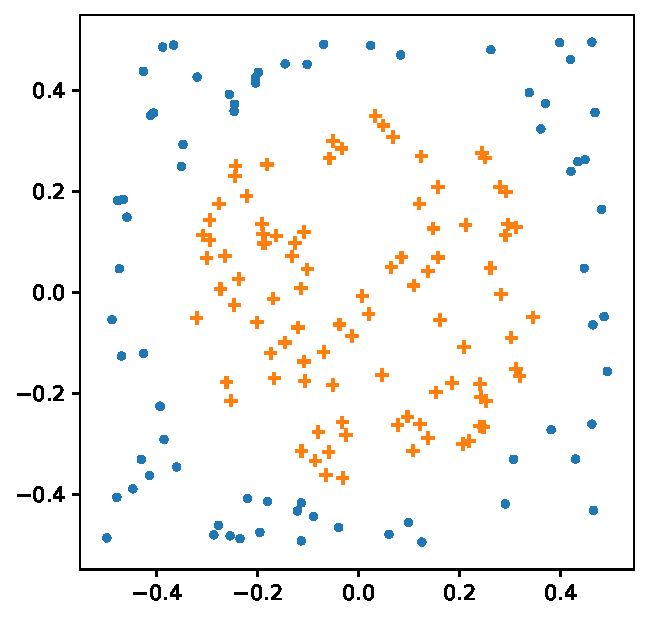
\includegraphics[width=0.49\linewidth]{figures/kernels-circle.pdf}
\hfill
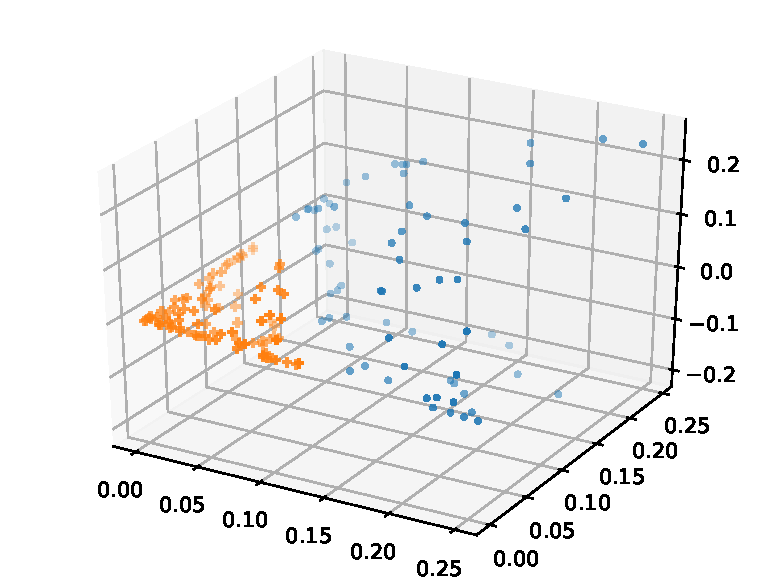
\includegraphics[width=0.49\linewidth]{figures/kernels-circle-3d.pdf}}
\caption{A two-feature binary classification data set (left), where the data points of different classes are not linearly separated. The same data set, where each point $\vect{x}$ was transformed through $\Phi(\vect{x})$, so that $\Phi(\vect{x})=\langle x_1^2, x_2^2, \sqrt{2}\ x_1 x_2\rangle$ (right).}
\label{fig:svm-circle}
\end{figure}

So, if, instead of using a dot product between two vectors $\x^\tr\x'$ in formulation of SVM, we can replace it with a $\kappa(\x,\x')=(\x^\tr \x')^2$. This substitution is called a kernel trick. The kernel trick avoids the explicit mapping that is needed to, say, get a linear model to learn a nonlinear function or decision boundary. For all $\x$ and $\x'$ in the input space, certain functions $\kappa(\x, \x')$ can be expressed as an inner product in another space. The function $\kappa$ is referred to as a kernel or a kernel function. Notice that the kernel trick allows us never to transform the data to the latent space, that is, never to use the transformation function $\Phi(\vect{x})$. In this way, the latent space could, in principle, have infinite dimensions, yet all we need is to compute the scalar product in this space. For any kernel, there is a corresponding function that transforms the data from original space to latent space, and there are some kernels where the required dimensionality of latent space is infinite. We will discuss various kernel functions and their properties a bit later in this chapter.

\begin{figure}
\centering{
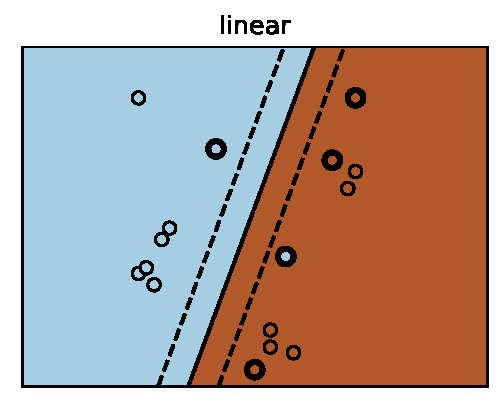
\includegraphics[width=0.32\linewidth]{figures/kernels-svm-linear.pdf}
\hfill
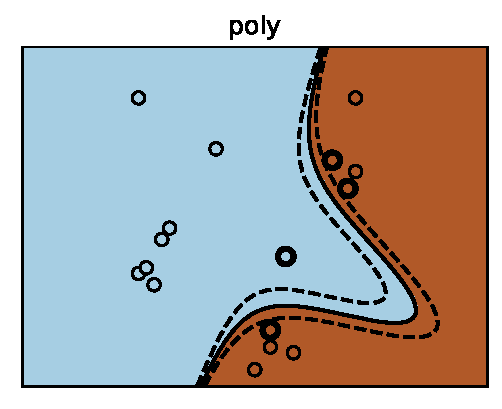
\includegraphics[width=0.32\linewidth]{figures/kernels-svm-poly.pdf}
\hfill
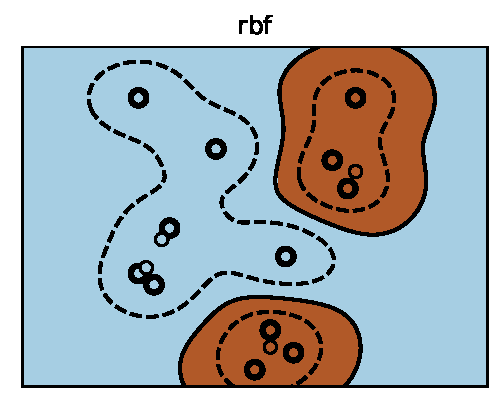
\includegraphics[width=0.32\linewidth]{figures/kernels-svm-rbf.pdf}
}
\caption{Classification in two-dimensional feature space shows decision boundaries of support vector machines with linear, polynomial ($n=3$), and Gaussian kernel. Double-circled data points are support vectors. Code for figures by Gaël Varoquaux.}
\label{fig:kernels-poly}
\end{figure}

\subsubsection*{Non-Linearly Separable Data}

If the data is not linearly separated, which is expected from any real data that contains some noise, the support vector machine that we have defined so far does not have any solution. For such cases, we need to introduce slack variables $\xi_i\geq 0$ such that slack is zero if the data instance is on or inside the correct margin boundary, or the slack is positive and equal to the distance to the corresponding margin. Notice that if $0<\xi_i\geq 1$ the point lies inside the margin, but on the corre side of decision boundary. To solve for this problem, we replace the hard constrains with {\em soft margin constraints} with the new objective, where, as before, we would like to maximize the margin with minimal use of slack:
$$ \min_{\vect{w},w_0,\vect{\xi}} {1\over 2}\norm{w}^2+C\sum_{i=1}^N\xi_i\ \ s.t.\ \xi_i\geq 0,\ y_i(\vect{w}^\tr \vect{x}_i+w_0)\geq 1-\xi_i,\ i=1\ldots N$$
The corresponding Lagrangian is
$$ L(\vect{w},w_0,\vect{\alpha})={1\over 2}\norm{w}^2 + C\sum_{i=1}^N\xi_i - \sum_{i=1}^N \alpha_i [y_i(\vect{w}^\tr \vect{x}_i+w_0)-1+\xi_i] -\sum_{i=1}^N\mu_i\xi_i$$
After computing the corresponding gradients and replacing the results in the primal Lagrangian, the dual form of Lagrangian is the same as before,
$$ \sum_{i=1}^N \alpha_i - {1\over 2}\sum_{i=1}^N\sum_{j=1}^N \alpha_i\alpha_j y_i y_j \vect{x}_i\vect{x}_j $$
with the only exception of a box constrain $0\leq\alpha_i\leq C$. Notice that the parameter $C$ is a regularization parameter that controls the number of errors we are willing to tolerate on the training set. This parameter is commonly defined as $C=1/(\nu N)$, where $0<\nu\leq 1$ is the fraction of misclassified points we allow during the training phase. This version of the algorithm is called $\nu$-SVM classifier.

\subsubsection*{Multi-Class Classification}

We have defined support vectors classifiers for supervised learning on binary classification data. Unlike some other approaches, like softmax for logistic regression, SVMs do not have a natural extension that would be appropriate to treat multi-class data. Standard approaches that solve multi-class problems through inference of a set of binary classifiers include a one-versus-all approach and one-versus-one approach. However, the problem to use them is that SVM, in its original formulation, is not a probabilistic classifier.

\subsubsection*{Choosing the Value of Hyper-Parameters}

Regularization parameters like $C$ and $\nu$ are parameters of the algorithm, that is, hyper-parameters that need to be set before the inference of the model. To search for the most appropriate value, we can use approaches such as the search over a fixed set of parameters and estimating their appropriateness through cross-validated accuracy on the training data. We then use the parameter value with the highest estimated accuracy to infer the model from the entire training set.

\subsubsection*{Hinge Loss}

An alternative derivation of support vector machine comes from the utility of {\em hige loss}, a variant of a loss function for binary classification, defined as:
$$ L_{\rm hinge}(y, \eta) = \max(0, 1-y\eta) = (1-y\eta)_{+} $$
Here, $\eta=f(\x)=\vect{w}^\tr x + w_0$ can be regarded as ``confidence'' in choosing label $y=1$. The overall objective is again to maximize the margin while minimizing the loss, therefore:
$$ \min_{\vect{w},w_0}{1\over 2}\norm{\vect{w}}^2 + C\sum_{i=1}^N(-y_i f(\vect{x}_i))_{+} $$
This objective function is non-differentiable because of the max term. We can replace this term with slack variables, and request in the revised objective that the slack is minimized. The new objective function 
$$ \min_{\vect{w},w_0,\vect{\xi}} {1\over 2}\norm{w}^2+C\sum_{i=1}^N\xi_i\ \ s.t.\ \xi_i\geq 0,\ y_i(\vect{w}^\tr \vect{x}_i+w_0)\geq 1-\xi_i,\ i=1\ldots N$$
is exactly the same as the one derived above, in the section on the treatment of non-linearably separable data.


\subsection*{Kernelized $k$-Nearest Neighbors}

$k$-nearest neighbor algorithms are based on distance, that is, they find the observations closest to the one we are predicting for. If using an Euclidean distance, this can be expressed in terms of inner products 
%
$$\lvert\lvert x, x' \rvert\rvert^2 =  \lvert\lvert x \rvert\rvert^2 + \lvert\lvert x' \rvert\rvert^2 - 2 \langle x, x'\rangle  =  \langle x, x\rangle^2 + \langle x', x'\rangle^2 - 2 \langle x, x'\rangle.$$
%
Thus, we can replace these dot products with a kernel, and in this way perform $k$-nearest neighbors in the feature space of a chosen kernel.

\subsection*{Support Vector Machines Regression}
% This is basically my review of 14.5.1; maybe some additional comments

Here, we motivate SVM with the problem of kernelized ridge regression, and actually with other approaches discussed so far that use the kernel trick, where the solution is not sparse. More precisely, the solution of kernelized ridge regression $\hat{\beta} = \sum \alpha_i \x_i$ and subsequently the predictions  $\hat{y}(x')  = \sum \alpha_i \kappa(\x',\x_i)$ depend on all training observations.

A key idea of SVMs is to introduce sparsity through the loss function. Vapnik proposed the \emph{epsilon insensitive loss function}:

$$L_\epsilon(y, \hat{y}) = |y-\hat{y}| - \epsilon\ {\rm if}\ |y-\hat{y}| \geq \epsilon\ {\rm and}\ 0\  {\rm otherwise}.$$
Basically, anything that has an absolute error less than $\epsilon$ is not penalized. The objective function we want to minimize is then

$$J = C\sum L_\epsilon(y_i, \hat{y}_i) + \frac{1}{2}\lvert\lvert \beta \rvert\rvert^2,$$
%
where $\hat{y}_i = f(\x_i) = \beta^T \x_i + \beta_0$ and $C = \frac{1}{\lambda}$ is a regularization constant.

This optimization problem is non-differentiable because of the absolute value in the loss function. Typically, it is reformulated as a constrained optimization problem by introducing slack variables $\xi$:

\begin{align*}
y_i - f(\x_i) & \leq + \epsilon + \xi_i^+, \\
y_i -  f(\x_i) & \geq - \epsilon - \xi_i^-.
\end{align*}

Now we can reformulate the objective function.

$$J = C\sum (\xi_i^+ + \xi_i^-) + \frac{1}{2}\lvert\lvert \b \rvert\rvert^2.$$
%
This is a quadratic function of $\b$ and we need to minimize it, subject to the above constraints and $\xi_i^+ \geq 0$, $\xi_i^- \geq 0$. Standard quadratic programming black-box solvers can be used.

If it is not immediately clear what we did with the slack variables: First, we deliberately put the  $f(\x_i)$ on the left-hand side of the inequality constraints above. This is to illustrate the fact that for observations that we can fit within $\epsilon$, the constraint will immediately be true, and both $\xi_i$ can be 0. For all other observations, one of the inequality constraints will be violated, but not both. So, one of the slack variables will be 0, and the other will be exactly the amount the fit exceeds $\epsilon$. This is what forces the $f(\x_i)$ as close to $y_i$ as possible, in the absolute sense; the only way to make $\xi_i$ as close to 0 as possible, again, in the absolute sense, is to make the $f(x_i)$ as close to $y_i$ as possible. That is, in the optimal solution, the sum of $\xi$ will be exactly the total sum of all exceedances of $\epsilon$), so by minimizing the one, we minimize the other. But we got rid of the absolute term.

The solution of the above optimization problem \citep{2012-Murphy} has, not surprisingly, the form
$$\hat{\b} = \sum_i \alpha_i \x_i,$$
%
where $\alpha_i \geq 0$. Notice that this solution is typically sparse, as most $\alpha_i = 0$. The $\x_i$ where $\alpha_i > 0$ are again called \emph{support vectors}. We should emphasize that the sparseness comes from the objective function ($\epsilon$). In practice, and depending on training data, we sometimes do get unlucky as it turns out that most $x_i$ from the training data are support vectors.

SVM regression is typically solved in its dual form. The form above is the primal form. The two forms are the same as the optimization problem is convex. The dual formulation is also where the result comes that the solution is a linear combination of observations, very similar to kernelized ridge regression.

As with kernelized ridge regression, the prediction for a new observation is
\begin{align*}
\hat{y}(x') & = \hat{\beta}_0 + x'^T\hat{\beta} \\
& = \hat{\beta}_0 + x'^T\sum \alpha_i x_i \\
& = \hat{\beta}_0 + \sum \alpha_i x'^Tx_i \\
& =  \hat{\beta}_0 + \sum \alpha_i \kappa(x', x_i)
\end{align*}
So, we can also use the kernel trick here and do SVM regression in a feature space determined by the choice of kernel.

\section*{Kernel Density Estimation}

Here, we will discuss on a substantially different kind of kernels, the so-called {\em smoothing kernels}. We will use the smoothing kernels to create non-parametric density estimates $p(\x)$, as well as for creating generative models for classification and regression of the form $p(y,\x)$.

A smoothing kernel is a one-argument function that satisfies the following properties:
$$ \int \kappa(x)dx = 1, $$
$$ \int x\kappa(x)dx = 0, $$
$$ \int x^2\kappa(x)dx > 0. $$

A simple example of a smoothing kernel is a {\em Gaussian kernel},
$$ \kappa(x)={1\over (2\pi)^{1\over 2}} e^{-x^2/2} $$
and we can control the width of the kernel by introducing a {\em bandwidth} parameter $h$:
$$ \kappa_h(x)={1\over h}\kappa{x\over h} $$
We can generalize this kernel to vector-valued inputs by defining an RBF kernel:
$$ \kappa_h(\x) = \kappa_h(\norm{\x}).$$

Kernel density estimators are different from, say, Gaussian mixture models, a parametric density estimator that requires speficying $K$ prototypes. An alternative is to allocate one cluster center per data point, so that the kernel density estimator, also called the {\em Parzen window density estimator} becomes
$$ \hat{p}(\x) = {1\over N}\sum_{i=1}^N \kappa_h(\x-\x_i).$$

The advantage of kernel density estimator over the parametric models is no need for model fitting and no need to pick the prototypes. However, we need to tune for the bandwidth, which can be performed by internal cross-validation. Notice also that the choice of $h$ influences the bias-variance tradeoff. More smoothing decreases bias but increases variance, less smoothing decreases variance but increases bias. The optimal point is somewhere in between. 


% \begin{itemize}
% \item What smoothing kernels are (14.7.1)
% \item Kernel density estimation and mention of histogram (14.7.2) NOTE: Murphy doesn't have an example of the important underlying principle - it's all about the bias-variance tradeoff. More smoothing decreases bias but increases variance, less smoothing decreases variance but increases bias. The optimal point is somewhere in between. You may want to refer to Wasserman's All of statistics: 20.1 (bias-variance tradeoff), 20.2 (histograms), 20.3 (KDE)
% \item OPTIONAL (kNN and kernel regression (14.7.3-4)
% \item LOESS (locally weighted regression) (14.7.5); this is pretty much state-of-the-art for 1D smoothing
% \end{itemize}

\printbibliography[heading=subbibliography]
\end{refsection}


